% ================================================================
% The printable version of latex/starters/targeted/KS3/circles/circlesIntroductoryStarters_retrieveAndConnect.tex
%
% This is the same deck, laid out to be handed out rather than put on
% the board. Every slide is shown as it stands before any answer is
% revealed, and 4 copies of it go on one page of A4, two by two, so
% that a printed page cuts into four question sheets.
%
%   made from           latex/starters/targeted/KS3/circles/circlesIntroductoryStarters_retrieveAndConnect.tex
%   slides on the sheet 4
%   copies of each      4, two by two on A4 landscape
%   printing rules      version 2
%
% Nothing was reworded and nothing was rewritten. Each slide is the slide
% from the deck, asked for at its first step, which is how the answers
% stay hidden.
%
% Please don't edit this file. It is written again from the one it was
% made from whenever that changes, so an edit here would be lost - edit
% that file instead and this one follows.
% ================================================================
% ================================================================
% The Retrieve and Connect version of latex/starters/targeted/KS3/circles/circlesIntroductoryStarters.tex
%
% This is the same deck as the one above, made by renaming the titles in it.
% Every slide that was a numbered starter is now titled
% "Retrieve and Connect", and the word is renamed wherever else a title
% used it. Nothing outside a title has been changed.
%
%   made from           latex/starters/targeted/KS3/circles/circlesIntroductoryStarters.tex
%   retitling rules     version 1
%
% Please don't edit this file. It is written again from the one it was
% made from whenever that changes, so an edit here would be lost - edit
% that file instead and this one follows.
% ================================================================
\documentclass{beamer}
\usepackage{tikz}
\usetikzlibrary{calc,arrows.meta,patterns}
\usepackage{xcolor}
\usepackage{multicol}
\usepackage{amsmath}

% ================================================================
% Answer-overlay helpers
% ================================================================
\newcommand{\ablank}[1]{%
  \alt<2>{\textcolor{red}{#1}}{\underline{\phantom{#1}}}%
}
\newcommand{\ashow}[1]{\uncover<2->{\textcolor{red}{\small #1}}}
\newcommand{\ashowq}[1]{\alt<2->{\textcolor{red}{\small #1}}{?}}

% Answers drawn straight on to a TikZ diagram, revealed on overlay 2 like \ashow.
% Space is reserved on overlay 1, so the diagram does not move between slides.
\usetikzlibrary{overlay-beamer-styles}
\tikzset{
  ans/.style     = {red, thick, visible on=<2->},
  ansfill/.style = {red!15, visible on=<2->},
  anslab/.style  = {red, font=\tiny, visible on=<2->},
}

\title{Circles: Parts, Perimeter \& Pi}
\author{}
\date{}

% ---------------------------------------------------------------
% Added so this deck prints four slides to a page. Nothing above
% this line was changed.
% ---------------------------------------------------------------
\usepackage{pgfpages}

% 4 slides to a sheet of A4, two by two, with a thin line round each
% so that the page can be cut up.
%
% Each slide keeps a margin of 1mm around it and no more, so the four fill
% the sheet and the pieces they cut into are as big as the paper allows. Only
% one direction actually comes out that tight: a slide is a different shape
% from a quarter of a sheet of A4, so it is scaled to fit and the slack it
% cannot use is left along whichever pair of edges it did not fill.
\pgfpagesuselayout{4 on 1}[a4paper,landscape,border shrink=1mm]
\pgfpageslogicalpageoptions{1}{border code=\pgfusepath{stroke}}
\pgfpageslogicalpageoptions{2}{border code=\pgfusepath{stroke}}
\pgfpageslogicalpageoptions{3}{border code=\pgfusepath{stroke}}
\pgfpageslogicalpageoptions{4}{border code=\pgfusepath{stroke}}

% There is nothing on paper to click, and a slide announcing a new section
% would sit between two copies of the same question and put every page after
% it out of step with the grid.
\setbeamertemplate{navigation symbols}{}
\AtBeginPart{}
\AtBeginSection{}
\AtBeginSubsection{}
\AtBeginSubsubsection{}
\begin{document}

\frame{\titlepage}

%------------------------------------------------
% SLIDE 1: Arithmetic, Lengths & Decimals (No Circles)
%------------------------------------------------
\begin{frame}<1>{Retrieve and Connect}


\begin{columns}

\column{0.3\textwidth}
\begin{center}
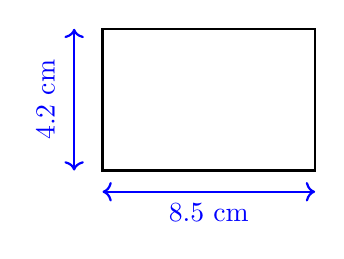
\begin{tikzpicture}[scale=0.9]
  % Rectangle for perimeter
  \draw[thick] (0,0) rectangle (3,2);
  \draw[blue, thick, <->] (0,-0.3) -- (3,-0.3);
  \node[blue] at (1.5,-0.6) {$8.5$ cm};
  \draw[blue, thick, <->] (-0.4,0) -- (-0.4,2);
  \node[blue, rotate=90] at (-0.8,1) {$4.2$ cm};
  
\end{tikzpicture}
\end{center}

\column{0.7\textwidth}
\small
\begin{enumerate}
    \begin{multicols}{2}
        \item $13 + 9 = \ashowq{22}$
        \item $5.8 - 1.9 = \ashowq{3.9}$
    \end{multicols}
    \begin{multicols}{2}
        \item $6 \times 8 = \ashowq{48}$
        \item $4 \times 3.5 \ \ashowq{14}$
  \end{multicols}
  \item Round $3.14159$ to 2 decimal places. \ashow{3.14}
  \item A pencil is $12.8$ cm long. How many millimetres is this? \ablank{128 mm}
\end{enumerate}

\begin{enumerate}
  \setcounter{enumi}{4}
  \item Find the perimeter of the rectangle shown. \ashow{25.4 cm}
  \item The perimeter of a square is $26$ cm. What is the length of one side? \ashow{6.5 cm}
  \item  The perimeter of an equilateral triangle is $12.9$ cm. 
    Find the length of one side, and then the perimeter of a regular hexagon with the same side length. \ashow{$4.3$ cm; hexagon: $25.8$ cm}
\end{enumerate}

\end{columns}
\end{frame}
\begin{frame}<1>{Retrieve and Connect}


\begin{columns}

\column{0.3\textwidth}
\begin{center}
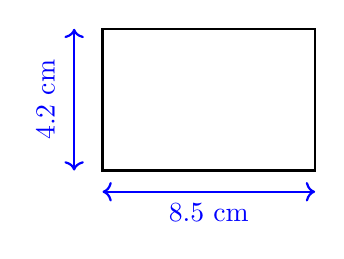
\begin{tikzpicture}[scale=0.9]
  % Rectangle for perimeter
  \draw[thick] (0,0) rectangle (3,2);
  \draw[blue, thick, <->] (0,-0.3) -- (3,-0.3);
  \node[blue] at (1.5,-0.6) {$8.5$ cm};
  \draw[blue, thick, <->] (-0.4,0) -- (-0.4,2);
  \node[blue, rotate=90] at (-0.8,1) {$4.2$ cm};
  
\end{tikzpicture}
\end{center}

\column{0.7\textwidth}
\small
\begin{enumerate}
    \begin{multicols}{2}
        \item $13 + 9 = \ashowq{22}$
        \item $5.8 - 1.9 = \ashowq{3.9}$
    \end{multicols}
    \begin{multicols}{2}
        \item $6 \times 8 = \ashowq{48}$
        \item $4 \times 3.5 \ \ashowq{14}$
  \end{multicols}
  \item Round $3.14159$ to 2 decimal places. \ashow{3.14}
  \item A pencil is $12.8$ cm long. How many millimetres is this? \ablank{128 mm}
\end{enumerate}

\begin{enumerate}
  \setcounter{enumi}{4}
  \item Find the perimeter of the rectangle shown. \ashow{25.4 cm}
  \item The perimeter of a square is $26$ cm. What is the length of one side? \ashow{6.5 cm}
  \item  The perimeter of an equilateral triangle is $12.9$ cm. 
    Find the length of one side, and then the perimeter of a regular hexagon with the same side length. \ashow{$4.3$ cm; hexagon: $25.8$ cm}
\end{enumerate}

\end{columns}
\end{frame}
\begin{frame}<1>{Retrieve and Connect}


\begin{columns}

\column{0.3\textwidth}
\begin{center}
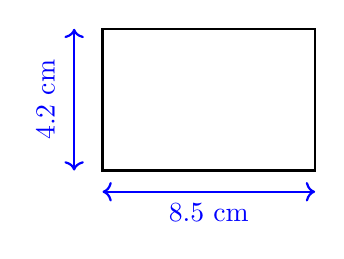
\begin{tikzpicture}[scale=0.9]
  % Rectangle for perimeter
  \draw[thick] (0,0) rectangle (3,2);
  \draw[blue, thick, <->] (0,-0.3) -- (3,-0.3);
  \node[blue] at (1.5,-0.6) {$8.5$ cm};
  \draw[blue, thick, <->] (-0.4,0) -- (-0.4,2);
  \node[blue, rotate=90] at (-0.8,1) {$4.2$ cm};
  
\end{tikzpicture}
\end{center}

\column{0.7\textwidth}
\small
\begin{enumerate}
    \begin{multicols}{2}
        \item $13 + 9 = \ashowq{22}$
        \item $5.8 - 1.9 = \ashowq{3.9}$
    \end{multicols}
    \begin{multicols}{2}
        \item $6 \times 8 = \ashowq{48}$
        \item $4 \times 3.5 \ \ashowq{14}$
  \end{multicols}
  \item Round $3.14159$ to 2 decimal places. \ashow{3.14}
  \item A pencil is $12.8$ cm long. How many millimetres is this? \ablank{128 mm}
\end{enumerate}

\begin{enumerate}
  \setcounter{enumi}{4}
  \item Find the perimeter of the rectangle shown. \ashow{25.4 cm}
  \item The perimeter of a square is $26$ cm. What is the length of one side? \ashow{6.5 cm}
  \item  The perimeter of an equilateral triangle is $12.9$ cm. 
    Find the length of one side, and then the perimeter of a regular hexagon with the same side length. \ashow{$4.3$ cm; hexagon: $25.8$ cm}
\end{enumerate}

\end{columns}
\end{frame}
\begin{frame}<1>{Retrieve and Connect}


\begin{columns}

\column{0.3\textwidth}
\begin{center}
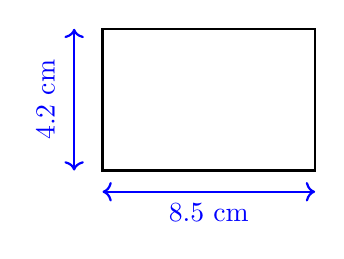
\begin{tikzpicture}[scale=0.9]
  % Rectangle for perimeter
  \draw[thick] (0,0) rectangle (3,2);
  \draw[blue, thick, <->] (0,-0.3) -- (3,-0.3);
  \node[blue] at (1.5,-0.6) {$8.5$ cm};
  \draw[blue, thick, <->] (-0.4,0) -- (-0.4,2);
  \node[blue, rotate=90] at (-0.8,1) {$4.2$ cm};
  
\end{tikzpicture}
\end{center}

\column{0.7\textwidth}
\small
\begin{enumerate}
    \begin{multicols}{2}
        \item $13 + 9 = \ashowq{22}$
        \item $5.8 - 1.9 = \ashowq{3.9}$
    \end{multicols}
    \begin{multicols}{2}
        \item $6 \times 8 = \ashowq{48}$
        \item $4 \times 3.5 \ \ashowq{14}$
  \end{multicols}
  \item Round $3.14159$ to 2 decimal places. \ashow{3.14}
  \item A pencil is $12.8$ cm long. How many millimetres is this? \ablank{128 mm}
\end{enumerate}

\begin{enumerate}
  \setcounter{enumi}{4}
  \item Find the perimeter of the rectangle shown. \ashow{25.4 cm}
  \item The perimeter of a square is $26$ cm. What is the length of one side? \ashow{6.5 cm}
  \item  The perimeter of an equilateral triangle is $12.9$ cm. 
    Find the length of one side, and then the perimeter of a regular hexagon with the same side length. \ashow{$4.3$ cm; hexagon: $25.8$ cm}
\end{enumerate}

\end{columns}
\end{frame}

%------------------------------------------------
% SLIDE 2: Arithmetic + Radius, Diameter, Chord
%------------------------------------------------
\begin{frame}<1>{Retrieve and Connect}
\vspace{-2em}
\begin{columns}

\column{0.3\textwidth}
\begin{center}
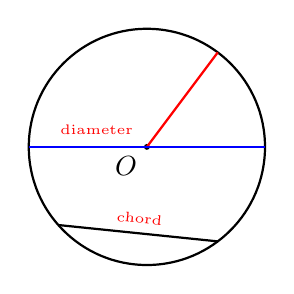
\begin{tikzpicture}[scale=0.75]
  % Circle
  \draw[thick] (0,0) circle (2cm);

  % Center
  \fill (0,0) circle (0.05);
  \node[below left] at (0,0) {$O$};

  % Radius
  \draw[red, thick] (0,0) -- (1.2,1.6);

  % Diameter
  \draw[blue, thick] (-2,0) -- (2,0);

  % Chord (not through center)
  \draw[thick] (-1.5,-1.323) -- (1.2,-1.6);

  % --- Q5 answer: name the lines on the diagram ---
  \node[anslab, above] at (-0.85,0.05) {diameter};
  \node[anslab, above, rotate=-6] at (-0.15,-1.46) {chord};
\end{tikzpicture}
\end{center}

\column{0.7\textwidth}
\small
\begin{enumerate}
\begin{multicols}{2}
  \item $24 \div 6$ \ashow{$=4$}
  \item $72 \div 8$ \ashow{$=9$}
  \end{multicols}
  \begin{multicols}{2}
  \item Double $15.5$ \ashow{$=31$}
  \item Halve $31.4$ \ashow{$=15.7$}
  \end{multicols}
  \item How many centimetres in $1.2$ metres? \ashow{120 cm}
  \item True or false? $2.5 \times 4 = 10$ \ashow{True}
\end{enumerate}

\begin{enumerate}
  \setcounter{enumi}{4}
  \item On the diagram, which line is the \textbf{diameter}? 
    How is it different from a chord? \ashow{A diameter passes through the centre.}
  \item If the radius of a circle is $7$ cm, what is its diameter? \ashow{14 cm}
  \item The diameter of a circle is $18$ mm. Find its radius. \ablank{9 mm}
  \item A chord of length $8$ cm is drawn inside a circle of radius $5$ cm.
    Is the chord a diameter? Why, or why not?. \ashow{No; a diameter would be $10$ cm.}
\end{enumerate}

\end{columns}
\end{frame}
\begin{frame}<1>{Retrieve and Connect}
\vspace{-2em}
\begin{columns}

\column{0.3\textwidth}
\begin{center}
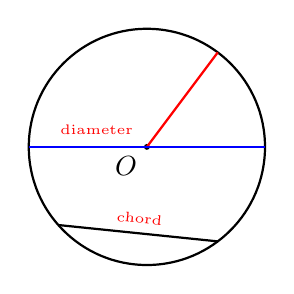
\begin{tikzpicture}[scale=0.75]
  % Circle
  \draw[thick] (0,0) circle (2cm);

  % Center
  \fill (0,0) circle (0.05);
  \node[below left] at (0,0) {$O$};

  % Radius
  \draw[red, thick] (0,0) -- (1.2,1.6);

  % Diameter
  \draw[blue, thick] (-2,0) -- (2,0);

  % Chord (not through center)
  \draw[thick] (-1.5,-1.323) -- (1.2,-1.6);

  % --- Q5 answer: name the lines on the diagram ---
  \node[anslab, above] at (-0.85,0.05) {diameter};
  \node[anslab, above, rotate=-6] at (-0.15,-1.46) {chord};
\end{tikzpicture}
\end{center}

\column{0.7\textwidth}
\small
\begin{enumerate}
\begin{multicols}{2}
  \item $24 \div 6$ \ashow{$=4$}
  \item $72 \div 8$ \ashow{$=9$}
  \end{multicols}
  \begin{multicols}{2}
  \item Double $15.5$ \ashow{$=31$}
  \item Halve $31.4$ \ashow{$=15.7$}
  \end{multicols}
  \item How many centimetres in $1.2$ metres? \ashow{120 cm}
  \item True or false? $2.5 \times 4 = 10$ \ashow{True}
\end{enumerate}

\begin{enumerate}
  \setcounter{enumi}{4}
  \item On the diagram, which line is the \textbf{diameter}? 
    How is it different from a chord? \ashow{A diameter passes through the centre.}
  \item If the radius of a circle is $7$ cm, what is its diameter? \ashow{14 cm}
  \item The diameter of a circle is $18$ mm. Find its radius. \ablank{9 mm}
  \item A chord of length $8$ cm is drawn inside a circle of radius $5$ cm.
    Is the chord a diameter? Why, or why not?. \ashow{No; a diameter would be $10$ cm.}
\end{enumerate}

\end{columns}
\end{frame}
\begin{frame}<1>{Retrieve and Connect}
\vspace{-2em}
\begin{columns}

\column{0.3\textwidth}
\begin{center}
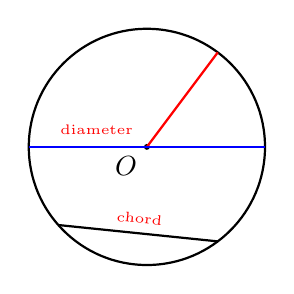
\begin{tikzpicture}[scale=0.75]
  % Circle
  \draw[thick] (0,0) circle (2cm);

  % Center
  \fill (0,0) circle (0.05);
  \node[below left] at (0,0) {$O$};

  % Radius
  \draw[red, thick] (0,0) -- (1.2,1.6);

  % Diameter
  \draw[blue, thick] (-2,0) -- (2,0);

  % Chord (not through center)
  \draw[thick] (-1.5,-1.323) -- (1.2,-1.6);

  % --- Q5 answer: name the lines on the diagram ---
  \node[anslab, above] at (-0.85,0.05) {diameter};
  \node[anslab, above, rotate=-6] at (-0.15,-1.46) {chord};
\end{tikzpicture}
\end{center}

\column{0.7\textwidth}
\small
\begin{enumerate}
\begin{multicols}{2}
  \item $24 \div 6$ \ashow{$=4$}
  \item $72 \div 8$ \ashow{$=9$}
  \end{multicols}
  \begin{multicols}{2}
  \item Double $15.5$ \ashow{$=31$}
  \item Halve $31.4$ \ashow{$=15.7$}
  \end{multicols}
  \item How many centimetres in $1.2$ metres? \ashow{120 cm}
  \item True or false? $2.5 \times 4 = 10$ \ashow{True}
\end{enumerate}

\begin{enumerate}
  \setcounter{enumi}{4}
  \item On the diagram, which line is the \textbf{diameter}? 
    How is it different from a chord? \ashow{A diameter passes through the centre.}
  \item If the radius of a circle is $7$ cm, what is its diameter? \ashow{14 cm}
  \item The diameter of a circle is $18$ mm. Find its radius. \ablank{9 mm}
  \item A chord of length $8$ cm is drawn inside a circle of radius $5$ cm.
    Is the chord a diameter? Why, or why not?. \ashow{No; a diameter would be $10$ cm.}
\end{enumerate}

\end{columns}
\end{frame}
\begin{frame}<1>{Retrieve and Connect}
\vspace{-2em}
\begin{columns}

\column{0.3\textwidth}
\begin{center}
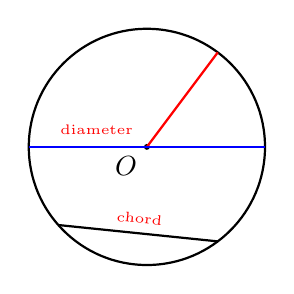
\begin{tikzpicture}[scale=0.75]
  % Circle
  \draw[thick] (0,0) circle (2cm);

  % Center
  \fill (0,0) circle (0.05);
  \node[below left] at (0,0) {$O$};

  % Radius
  \draw[red, thick] (0,0) -- (1.2,1.6);

  % Diameter
  \draw[blue, thick] (-2,0) -- (2,0);

  % Chord (not through center)
  \draw[thick] (-1.5,-1.323) -- (1.2,-1.6);

  % --- Q5 answer: name the lines on the diagram ---
  \node[anslab, above] at (-0.85,0.05) {diameter};
  \node[anslab, above, rotate=-6] at (-0.15,-1.46) {chord};
\end{tikzpicture}
\end{center}

\column{0.7\textwidth}
\small
\begin{enumerate}
\begin{multicols}{2}
  \item $24 \div 6$ \ashow{$=4$}
  \item $72 \div 8$ \ashow{$=9$}
  \end{multicols}
  \begin{multicols}{2}
  \item Double $15.5$ \ashow{$=31$}
  \item Halve $31.4$ \ashow{$=15.7$}
  \end{multicols}
  \item How many centimetres in $1.2$ metres? \ashow{120 cm}
  \item True or false? $2.5 \times 4 = 10$ \ashow{True}
\end{enumerate}

\begin{enumerate}
  \setcounter{enumi}{4}
  \item On the diagram, which line is the \textbf{diameter}? 
    How is it different from a chord? \ashow{A diameter passes through the centre.}
  \item If the radius of a circle is $7$ cm, what is its diameter? \ashow{14 cm}
  \item The diameter of a circle is $18$ mm. Find its radius. \ablank{9 mm}
  \item A chord of length $8$ cm is drawn inside a circle of radius $5$ cm.
    Is the chord a diameter? Why, or why not?. \ashow{No; a diameter would be $10$ cm.}
\end{enumerate}

\end{columns}
\end{frame}

%------------------------------------------------
% SLIDE 3: Arithmetic + Segments, Sectors, Arcs, Tangents
%------------------------------------------------
\begin{frame}<1>{Retrieve and Connect}

\vspace{-2em}

\begin{columns}

\column{0.35\textwidth}

\begin{center}
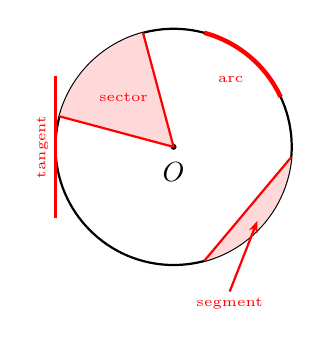
\begin{tikzpicture}[scale=0.75]
  % Circle
  \draw[thick] (0,0) circle (2cm);
  \fill (0,0) circle (0.05);
  \node[below] at (0,-0.1) {$O$};

  % --- Q6 answers: drawn on the circle ---
  % Sector
  \fill[ansfill] (0,0) -- (105:2) arc (105:165:2) -- cycle;
  \draw[ans] (0,0) -- (105:2);
  \draw[ans] (0,0) -- (165:2);
  \node[anslab] at (135:1.2) {sector};

  % Arc
  \draw[ans, ultra thick] (25:2) arc (25:75:2);
  \node[anslab] at (50:1.5) {arc};

  % Tangent
  \draw[ans] (-2,-1.2) -- (-2,1.2);
  \node[anslab, rotate=90] at (-2.22,0) {tangent};

  % Segment
  \fill[ansfill] (-75:2) arc (-75:-5:2) -- cycle;
  \draw[ans] (-75:2) -- (-5:2);
  \draw[ans, -{Stealth[length=1.5mm]}] (0.95,-2.45) -- (1.42,-1.25);
  \node[anslab] at (0.95,-2.65) {segment};
\end{tikzpicture}

\vspace{3em}

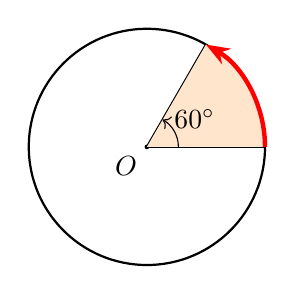
\begin{tikzpicture}[scale=1]
  % Circle
  \draw[thick] (0,0) circle (1.5cm);
  
  % Centre
  \fill (0,0) circle (0.03);
  \node[below left] at (0,0) {$O$};
  
  % Radii that bound the 60° sector
  \draw[thick] (0,0) -- (0:1.5);          % right horizontal radius
  \draw[thick] (0,0) -- (60:1.5);         % radius at 60°
  

  
  % Optional: shade the sector lightly
  \fill[orange!20] (0,0) -- (0:1.5) arc (0:60:1.5) -- cycle;

    % Highlight the arc (thick, coloured, with arrow)
  \draw[red, ultra thick, -{Stealth[length=3mm]}] 
    (0:1.5) arc (0:60:1.5);
  
  % Angle arc and label
  \draw[->] (0.4,0) arc (0:60:0.4);
  \node at (30:0.7) {$60^\circ$};
  
\end{tikzpicture}

\end{center}


\column{0.65\textwidth}
\small
\begin{enumerate}
\begin{multicols}{2}
  \item $3.2 \times 5$ \ashow{$=16$}
  \item $1.8 \times 4$ \ashow{$=7.2$}
  \end{multicols}
  \begin{multicols}{2}
    \item  $45 \div 10$ \ashow{$=4.5$}
    \item $90 \div 100$ \ashow{$=0.9$}
  \end{multicols}
  \item What is $\frac{1}{4}$ of $360^\circ$? \ashow{$90^\circ$}
\end{enumerate}

\begin{enumerate}
  \setcounter{enumi}{5}
  \item Copy the diagram, and draw with labels:
    \begin{multicols}{2}
    \begin{itemize}
      \item A sector
      \item An arc
      \item A tangent
      \item A segment
    \end{itemize}
    \end{multicols}
  \item If the radius is $6$ cm, what is the whole circumference? (Use $\pi \approx 3.14$) \ashow{$37.68$ cm}
  \item For the sector shown, what fraction of the circumference is the arc length? Calculate the arc length if the whole circle has a circumference of 24cm. \ashow{$\frac{1}{6}$; $4$ cm}

\end{enumerate}

\end{columns}
\end{frame}
\begin{frame}<1>{Retrieve and Connect}

\vspace{-2em}

\begin{columns}

\column{0.35\textwidth}

\begin{center}
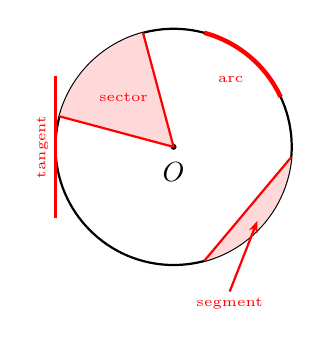
\begin{tikzpicture}[scale=0.75]
  % Circle
  \draw[thick] (0,0) circle (2cm);
  \fill (0,0) circle (0.05);
  \node[below] at (0,-0.1) {$O$};

  % --- Q6 answers: drawn on the circle ---
  % Sector
  \fill[ansfill] (0,0) -- (105:2) arc (105:165:2) -- cycle;
  \draw[ans] (0,0) -- (105:2);
  \draw[ans] (0,0) -- (165:2);
  \node[anslab] at (135:1.2) {sector};

  % Arc
  \draw[ans, ultra thick] (25:2) arc (25:75:2);
  \node[anslab] at (50:1.5) {arc};

  % Tangent
  \draw[ans] (-2,-1.2) -- (-2,1.2);
  \node[anslab, rotate=90] at (-2.22,0) {tangent};

  % Segment
  \fill[ansfill] (-75:2) arc (-75:-5:2) -- cycle;
  \draw[ans] (-75:2) -- (-5:2);
  \draw[ans, -{Stealth[length=1.5mm]}] (0.95,-2.45) -- (1.42,-1.25);
  \node[anslab] at (0.95,-2.65) {segment};
\end{tikzpicture}

\vspace{3em}

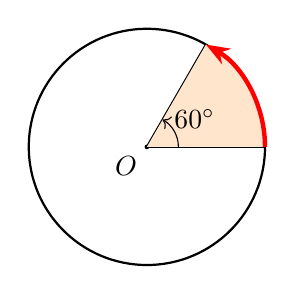
\begin{tikzpicture}[scale=1]
  % Circle
  \draw[thick] (0,0) circle (1.5cm);
  
  % Centre
  \fill (0,0) circle (0.03);
  \node[below left] at (0,0) {$O$};
  
  % Radii that bound the 60° sector
  \draw[thick] (0,0) -- (0:1.5);          % right horizontal radius
  \draw[thick] (0,0) -- (60:1.5);         % radius at 60°
  

  
  % Optional: shade the sector lightly
  \fill[orange!20] (0,0) -- (0:1.5) arc (0:60:1.5) -- cycle;

    % Highlight the arc (thick, coloured, with arrow)
  \draw[red, ultra thick, -{Stealth[length=3mm]}] 
    (0:1.5) arc (0:60:1.5);
  
  % Angle arc and label
  \draw[->] (0.4,0) arc (0:60:0.4);
  \node at (30:0.7) {$60^\circ$};
  
\end{tikzpicture}

\end{center}


\column{0.65\textwidth}
\small
\begin{enumerate}
\begin{multicols}{2}
  \item $3.2 \times 5$ \ashow{$=16$}
  \item $1.8 \times 4$ \ashow{$=7.2$}
  \end{multicols}
  \begin{multicols}{2}
    \item  $45 \div 10$ \ashow{$=4.5$}
    \item $90 \div 100$ \ashow{$=0.9$}
  \end{multicols}
  \item What is $\frac{1}{4}$ of $360^\circ$? \ashow{$90^\circ$}
\end{enumerate}

\begin{enumerate}
  \setcounter{enumi}{5}
  \item Copy the diagram, and draw with labels:
    \begin{multicols}{2}
    \begin{itemize}
      \item A sector
      \item An arc
      \item A tangent
      \item A segment
    \end{itemize}
    \end{multicols}
  \item If the radius is $6$ cm, what is the whole circumference? (Use $\pi \approx 3.14$) \ashow{$37.68$ cm}
  \item For the sector shown, what fraction of the circumference is the arc length? Calculate the arc length if the whole circle has a circumference of 24cm. \ashow{$\frac{1}{6}$; $4$ cm}

\end{enumerate}

\end{columns}
\end{frame}
\begin{frame}<1>{Retrieve and Connect}

\vspace{-2em}

\begin{columns}

\column{0.35\textwidth}

\begin{center}
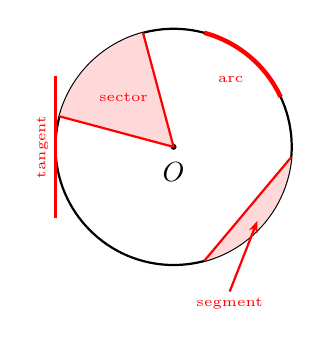
\begin{tikzpicture}[scale=0.75]
  % Circle
  \draw[thick] (0,0) circle (2cm);
  \fill (0,0) circle (0.05);
  \node[below] at (0,-0.1) {$O$};

  % --- Q6 answers: drawn on the circle ---
  % Sector
  \fill[ansfill] (0,0) -- (105:2) arc (105:165:2) -- cycle;
  \draw[ans] (0,0) -- (105:2);
  \draw[ans] (0,0) -- (165:2);
  \node[anslab] at (135:1.2) {sector};

  % Arc
  \draw[ans, ultra thick] (25:2) arc (25:75:2);
  \node[anslab] at (50:1.5) {arc};

  % Tangent
  \draw[ans] (-2,-1.2) -- (-2,1.2);
  \node[anslab, rotate=90] at (-2.22,0) {tangent};

  % Segment
  \fill[ansfill] (-75:2) arc (-75:-5:2) -- cycle;
  \draw[ans] (-75:2) -- (-5:2);
  \draw[ans, -{Stealth[length=1.5mm]}] (0.95,-2.45) -- (1.42,-1.25);
  \node[anslab] at (0.95,-2.65) {segment};
\end{tikzpicture}

\vspace{3em}

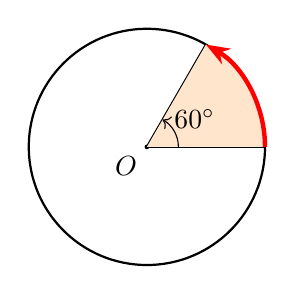
\begin{tikzpicture}[scale=1]
  % Circle
  \draw[thick] (0,0) circle (1.5cm);
  
  % Centre
  \fill (0,0) circle (0.03);
  \node[below left] at (0,0) {$O$};
  
  % Radii that bound the 60° sector
  \draw[thick] (0,0) -- (0:1.5);          % right horizontal radius
  \draw[thick] (0,0) -- (60:1.5);         % radius at 60°
  

  
  % Optional: shade the sector lightly
  \fill[orange!20] (0,0) -- (0:1.5) arc (0:60:1.5) -- cycle;

    % Highlight the arc (thick, coloured, with arrow)
  \draw[red, ultra thick, -{Stealth[length=3mm]}] 
    (0:1.5) arc (0:60:1.5);
  
  % Angle arc and label
  \draw[->] (0.4,0) arc (0:60:0.4);
  \node at (30:0.7) {$60^\circ$};
  
\end{tikzpicture}

\end{center}


\column{0.65\textwidth}
\small
\begin{enumerate}
\begin{multicols}{2}
  \item $3.2 \times 5$ \ashow{$=16$}
  \item $1.8 \times 4$ \ashow{$=7.2$}
  \end{multicols}
  \begin{multicols}{2}
    \item  $45 \div 10$ \ashow{$=4.5$}
    \item $90 \div 100$ \ashow{$=0.9$}
  \end{multicols}
  \item What is $\frac{1}{4}$ of $360^\circ$? \ashow{$90^\circ$}
\end{enumerate}

\begin{enumerate}
  \setcounter{enumi}{5}
  \item Copy the diagram, and draw with labels:
    \begin{multicols}{2}
    \begin{itemize}
      \item A sector
      \item An arc
      \item A tangent
      \item A segment
    \end{itemize}
    \end{multicols}
  \item If the radius is $6$ cm, what is the whole circumference? (Use $\pi \approx 3.14$) \ashow{$37.68$ cm}
  \item For the sector shown, what fraction of the circumference is the arc length? Calculate the arc length if the whole circle has a circumference of 24cm. \ashow{$\frac{1}{6}$; $4$ cm}

\end{enumerate}

\end{columns}
\end{frame}
\begin{frame}<1>{Retrieve and Connect}

\vspace{-2em}

\begin{columns}

\column{0.35\textwidth}

\begin{center}
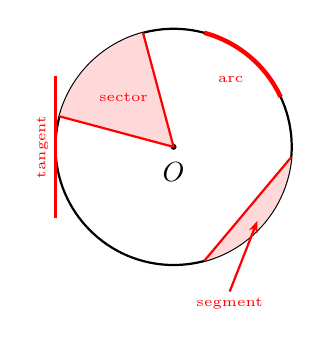
\begin{tikzpicture}[scale=0.75]
  % Circle
  \draw[thick] (0,0) circle (2cm);
  \fill (0,0) circle (0.05);
  \node[below] at (0,-0.1) {$O$};

  % --- Q6 answers: drawn on the circle ---
  % Sector
  \fill[ansfill] (0,0) -- (105:2) arc (105:165:2) -- cycle;
  \draw[ans] (0,0) -- (105:2);
  \draw[ans] (0,0) -- (165:2);
  \node[anslab] at (135:1.2) {sector};

  % Arc
  \draw[ans, ultra thick] (25:2) arc (25:75:2);
  \node[anslab] at (50:1.5) {arc};

  % Tangent
  \draw[ans] (-2,-1.2) -- (-2,1.2);
  \node[anslab, rotate=90] at (-2.22,0) {tangent};

  % Segment
  \fill[ansfill] (-75:2) arc (-75:-5:2) -- cycle;
  \draw[ans] (-75:2) -- (-5:2);
  \draw[ans, -{Stealth[length=1.5mm]}] (0.95,-2.45) -- (1.42,-1.25);
  \node[anslab] at (0.95,-2.65) {segment};
\end{tikzpicture}

\vspace{3em}

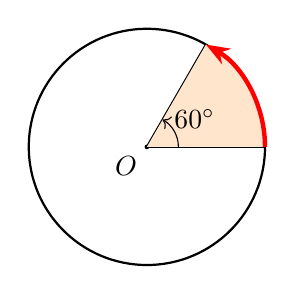
\begin{tikzpicture}[scale=1]
  % Circle
  \draw[thick] (0,0) circle (1.5cm);
  
  % Centre
  \fill (0,0) circle (0.03);
  \node[below left] at (0,0) {$O$};
  
  % Radii that bound the 60° sector
  \draw[thick] (0,0) -- (0:1.5);          % right horizontal radius
  \draw[thick] (0,0) -- (60:1.5);         % radius at 60°
  

  
  % Optional: shade the sector lightly
  \fill[orange!20] (0,0) -- (0:1.5) arc (0:60:1.5) -- cycle;

    % Highlight the arc (thick, coloured, with arrow)
  \draw[red, ultra thick, -{Stealth[length=3mm]}] 
    (0:1.5) arc (0:60:1.5);
  
  % Angle arc and label
  \draw[->] (0.4,0) arc (0:60:0.4);
  \node at (30:0.7) {$60^\circ$};
  
\end{tikzpicture}

\end{center}


\column{0.65\textwidth}
\small
\begin{enumerate}
\begin{multicols}{2}
  \item $3.2 \times 5$ \ashow{$=16$}
  \item $1.8 \times 4$ \ashow{$=7.2$}
  \end{multicols}
  \begin{multicols}{2}
    \item  $45 \div 10$ \ashow{$=4.5$}
    \item $90 \div 100$ \ashow{$=0.9$}
  \end{multicols}
  \item What is $\frac{1}{4}$ of $360^\circ$? \ashow{$90^\circ$}
\end{enumerate}

\begin{enumerate}
  \setcounter{enumi}{5}
  \item Copy the diagram, and draw with labels:
    \begin{multicols}{2}
    \begin{itemize}
      \item A sector
      \item An arc
      \item A tangent
      \item A segment
    \end{itemize}
    \end{multicols}
  \item If the radius is $6$ cm, what is the whole circumference? (Use $\pi \approx 3.14$) \ashow{$37.68$ cm}
  \item For the sector shown, what fraction of the circumference is the arc length? Calculate the arc length if the whole circle has a circumference of 24cm. \ashow{$\frac{1}{6}$; $4$ cm}

\end{enumerate}

\end{columns}
\end{frame}

%------------------------------------------------
% SLIDE 4: Arithmetic + Labelling, Pi, Diameter
%------------------------------------------------
\begin{frame}<1>{Retrieve and Connect}

\vspace{-2em}

\begin{columns}

\column{0.3\textwidth}
\begin{center}
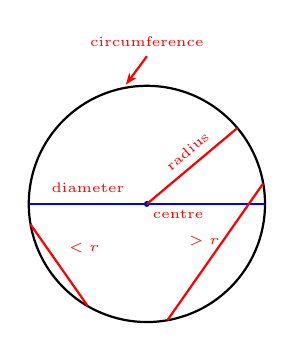
\begin{tikzpicture}[scale=0.75]
  % Circle with labels
  \draw[thick] (0,0) circle (2cm);
  \fill (0,0) circle (0.05);

  \draw[blue, thick] (-2,0) -- (2,0);

  \draw[red, thick] (0,0) -- (40:2);

  % --- Q8 answer: label the parts on the diagram ---
  \node[anslab, below right, inner sep=2pt] at (0,0) {centre};
  \node[anslab, above, rotate=40] at (40:1.1) {radius};
  \node[anslab, above] at (-1,0.02) {diameter};
  \draw[ans, -{Stealth[length=1.5mm]}] (0,2.5) -- (100:2.05);
  \node[anslab, above] at (0,2.5) {circumference};

  % --- Q9 answer: a chord shorter than the radius ---
  \draw[ans] (190:2) -- (240:2);
  \node[anslab] at (215:1.3) {$<r$};

  % --- Q10 answer: a chord longer than the radius ---
  \draw[ans] (-80:2) -- (10:2);
  \node[anslab] at (-33:1.15) {$>r$};
\end{tikzpicture}

\end{center}

\column{0.7\textwidth}
\small
\begin{enumerate}
\begin{multicols}{2}
  \item $12 \times 3 $ \ashow{$=36$}
  \item $4 \times 3.14$ \ashow{$=12.56$}
\end{multicols}
\begin{multicols}{2}
  \item $6.28 \div 2 $ \ashow{$=3.14$} 
  \item $ 9.42 \div 3$ \ashow{$=3.14$}
  \end{multicols}
  \item Round $3.14159265$ to 3 decimal places. \ashow{3.142}
  \begin{multicols}{2}
  \item Double $3.14$ \ashow{$=6.28$}
  \item halve $12.56$ \ashow{$=6.28$}
  \end{multicols}
\end{enumerate}
\vspace{-0.5em}
\begin{enumerate}
  \setcounter{enumi}{7}
  \item Copy and label on the diagram: 
    centre, radius, diameter, circumference.
    \item Draw a chord on the diagram shorter than the radius
    \item Draw a chord on the diagram longer than the radius
  
  \item If the diameter is $8$ cm, what is:
    \begin{itemize}
      \item the radius? \ashow{$4$ cm}
      \item the circumference? ($\pi \approx 3.14$) \ashow{$25.12$ cm}
    \end{itemize}
 
\end{enumerate}

\end{columns}
\end{frame}
\begin{frame}<1>{Retrieve and Connect}

\vspace{-2em}

\begin{columns}

\column{0.3\textwidth}
\begin{center}
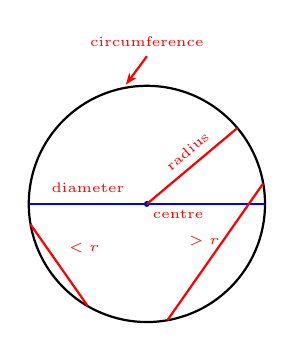
\begin{tikzpicture}[scale=0.75]
  % Circle with labels
  \draw[thick] (0,0) circle (2cm);
  \fill (0,0) circle (0.05);

  \draw[blue, thick] (-2,0) -- (2,0);

  \draw[red, thick] (0,0) -- (40:2);

  % --- Q8 answer: label the parts on the diagram ---
  \node[anslab, below right, inner sep=2pt] at (0,0) {centre};
  \node[anslab, above, rotate=40] at (40:1.1) {radius};
  \node[anslab, above] at (-1,0.02) {diameter};
  \draw[ans, -{Stealth[length=1.5mm]}] (0,2.5) -- (100:2.05);
  \node[anslab, above] at (0,2.5) {circumference};

  % --- Q9 answer: a chord shorter than the radius ---
  \draw[ans] (190:2) -- (240:2);
  \node[anslab] at (215:1.3) {$<r$};

  % --- Q10 answer: a chord longer than the radius ---
  \draw[ans] (-80:2) -- (10:2);
  \node[anslab] at (-33:1.15) {$>r$};
\end{tikzpicture}

\end{center}

\column{0.7\textwidth}
\small
\begin{enumerate}
\begin{multicols}{2}
  \item $12 \times 3 $ \ashow{$=36$}
  \item $4 \times 3.14$ \ashow{$=12.56$}
\end{multicols}
\begin{multicols}{2}
  \item $6.28 \div 2 $ \ashow{$=3.14$} 
  \item $ 9.42 \div 3$ \ashow{$=3.14$}
  \end{multicols}
  \item Round $3.14159265$ to 3 decimal places. \ashow{3.142}
  \begin{multicols}{2}
  \item Double $3.14$ \ashow{$=6.28$}
  \item halve $12.56$ \ashow{$=6.28$}
  \end{multicols}
\end{enumerate}
\vspace{-0.5em}
\begin{enumerate}
  \setcounter{enumi}{7}
  \item Copy and label on the diagram: 
    centre, radius, diameter, circumference.
    \item Draw a chord on the diagram shorter than the radius
    \item Draw a chord on the diagram longer than the radius
  
  \item If the diameter is $8$ cm, what is:
    \begin{itemize}
      \item the radius? \ashow{$4$ cm}
      \item the circumference? ($\pi \approx 3.14$) \ashow{$25.12$ cm}
    \end{itemize}
 
\end{enumerate}

\end{columns}
\end{frame}
\begin{frame}<1>{Retrieve and Connect}

\vspace{-2em}

\begin{columns}

\column{0.3\textwidth}
\begin{center}
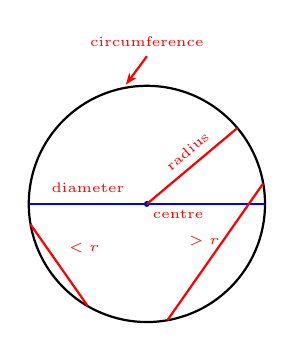
\begin{tikzpicture}[scale=0.75]
  % Circle with labels
  \draw[thick] (0,0) circle (2cm);
  \fill (0,0) circle (0.05);

  \draw[blue, thick] (-2,0) -- (2,0);

  \draw[red, thick] (0,0) -- (40:2);

  % --- Q8 answer: label the parts on the diagram ---
  \node[anslab, below right, inner sep=2pt] at (0,0) {centre};
  \node[anslab, above, rotate=40] at (40:1.1) {radius};
  \node[anslab, above] at (-1,0.02) {diameter};
  \draw[ans, -{Stealth[length=1.5mm]}] (0,2.5) -- (100:2.05);
  \node[anslab, above] at (0,2.5) {circumference};

  % --- Q9 answer: a chord shorter than the radius ---
  \draw[ans] (190:2) -- (240:2);
  \node[anslab] at (215:1.3) {$<r$};

  % --- Q10 answer: a chord longer than the radius ---
  \draw[ans] (-80:2) -- (10:2);
  \node[anslab] at (-33:1.15) {$>r$};
\end{tikzpicture}

\end{center}

\column{0.7\textwidth}
\small
\begin{enumerate}
\begin{multicols}{2}
  \item $12 \times 3 $ \ashow{$=36$}
  \item $4 \times 3.14$ \ashow{$=12.56$}
\end{multicols}
\begin{multicols}{2}
  \item $6.28 \div 2 $ \ashow{$=3.14$} 
  \item $ 9.42 \div 3$ \ashow{$=3.14$}
  \end{multicols}
  \item Round $3.14159265$ to 3 decimal places. \ashow{3.142}
  \begin{multicols}{2}
  \item Double $3.14$ \ashow{$=6.28$}
  \item halve $12.56$ \ashow{$=6.28$}
  \end{multicols}
\end{enumerate}
\vspace{-0.5em}
\begin{enumerate}
  \setcounter{enumi}{7}
  \item Copy and label on the diagram: 
    centre, radius, diameter, circumference.
    \item Draw a chord on the diagram shorter than the radius
    \item Draw a chord on the diagram longer than the radius
  
  \item If the diameter is $8$ cm, what is:
    \begin{itemize}
      \item the radius? \ashow{$4$ cm}
      \item the circumference? ($\pi \approx 3.14$) \ashow{$25.12$ cm}
    \end{itemize}
 
\end{enumerate}

\end{columns}
\end{frame}
\begin{frame}<1>{Retrieve and Connect}

\vspace{-2em}

\begin{columns}

\column{0.3\textwidth}
\begin{center}
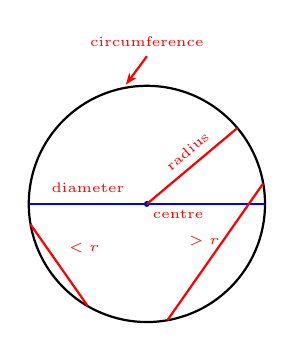
\begin{tikzpicture}[scale=0.75]
  % Circle with labels
  \draw[thick] (0,0) circle (2cm);
  \fill (0,0) circle (0.05);

  \draw[blue, thick] (-2,0) -- (2,0);

  \draw[red, thick] (0,0) -- (40:2);

  % --- Q8 answer: label the parts on the diagram ---
  \node[anslab, below right, inner sep=2pt] at (0,0) {centre};
  \node[anslab, above, rotate=40] at (40:1.1) {radius};
  \node[anslab, above] at (-1,0.02) {diameter};
  \draw[ans, -{Stealth[length=1.5mm]}] (0,2.5) -- (100:2.05);
  \node[anslab, above] at (0,2.5) {circumference};

  % --- Q9 answer: a chord shorter than the radius ---
  \draw[ans] (190:2) -- (240:2);
  \node[anslab] at (215:1.3) {$<r$};

  % --- Q10 answer: a chord longer than the radius ---
  \draw[ans] (-80:2) -- (10:2);
  \node[anslab] at (-33:1.15) {$>r$};
\end{tikzpicture}

\end{center}

\column{0.7\textwidth}
\small
\begin{enumerate}
\begin{multicols}{2}
  \item $12 \times 3 $ \ashow{$=36$}
  \item $4 \times 3.14$ \ashow{$=12.56$}
\end{multicols}
\begin{multicols}{2}
  \item $6.28 \div 2 $ \ashow{$=3.14$} 
  \item $ 9.42 \div 3$ \ashow{$=3.14$}
  \end{multicols}
  \item Round $3.14159265$ to 3 decimal places. \ashow{3.142}
  \begin{multicols}{2}
  \item Double $3.14$ \ashow{$=6.28$}
  \item halve $12.56$ \ashow{$=6.28$}
  \end{multicols}
\end{enumerate}
\vspace{-0.5em}
\begin{enumerate}
  \setcounter{enumi}{7}
  \item Copy and label on the diagram: 
    centre, radius, diameter, circumference.
    \item Draw a chord on the diagram shorter than the radius
    \item Draw a chord on the diagram longer than the radius
  
  \item If the diameter is $8$ cm, what is:
    \begin{itemize}
      \item the radius? \ashow{$4$ cm}
      \item the circumference? ($\pi \approx 3.14$) \ashow{$25.12$ cm}
    \end{itemize}
 
\end{enumerate}

\end{columns}
\end{frame}

\end{document}
